\section{BankHandler Class Reference}
\label{classBankHandler}\index{BankHandler@{BankHandler}}
{\tt \#include $<$bank\_\-handler.h$>$}

Inheritance diagram for BankHandler:\nopagebreak
\begin{figure}[H]
\begin{center}
\leavevmode
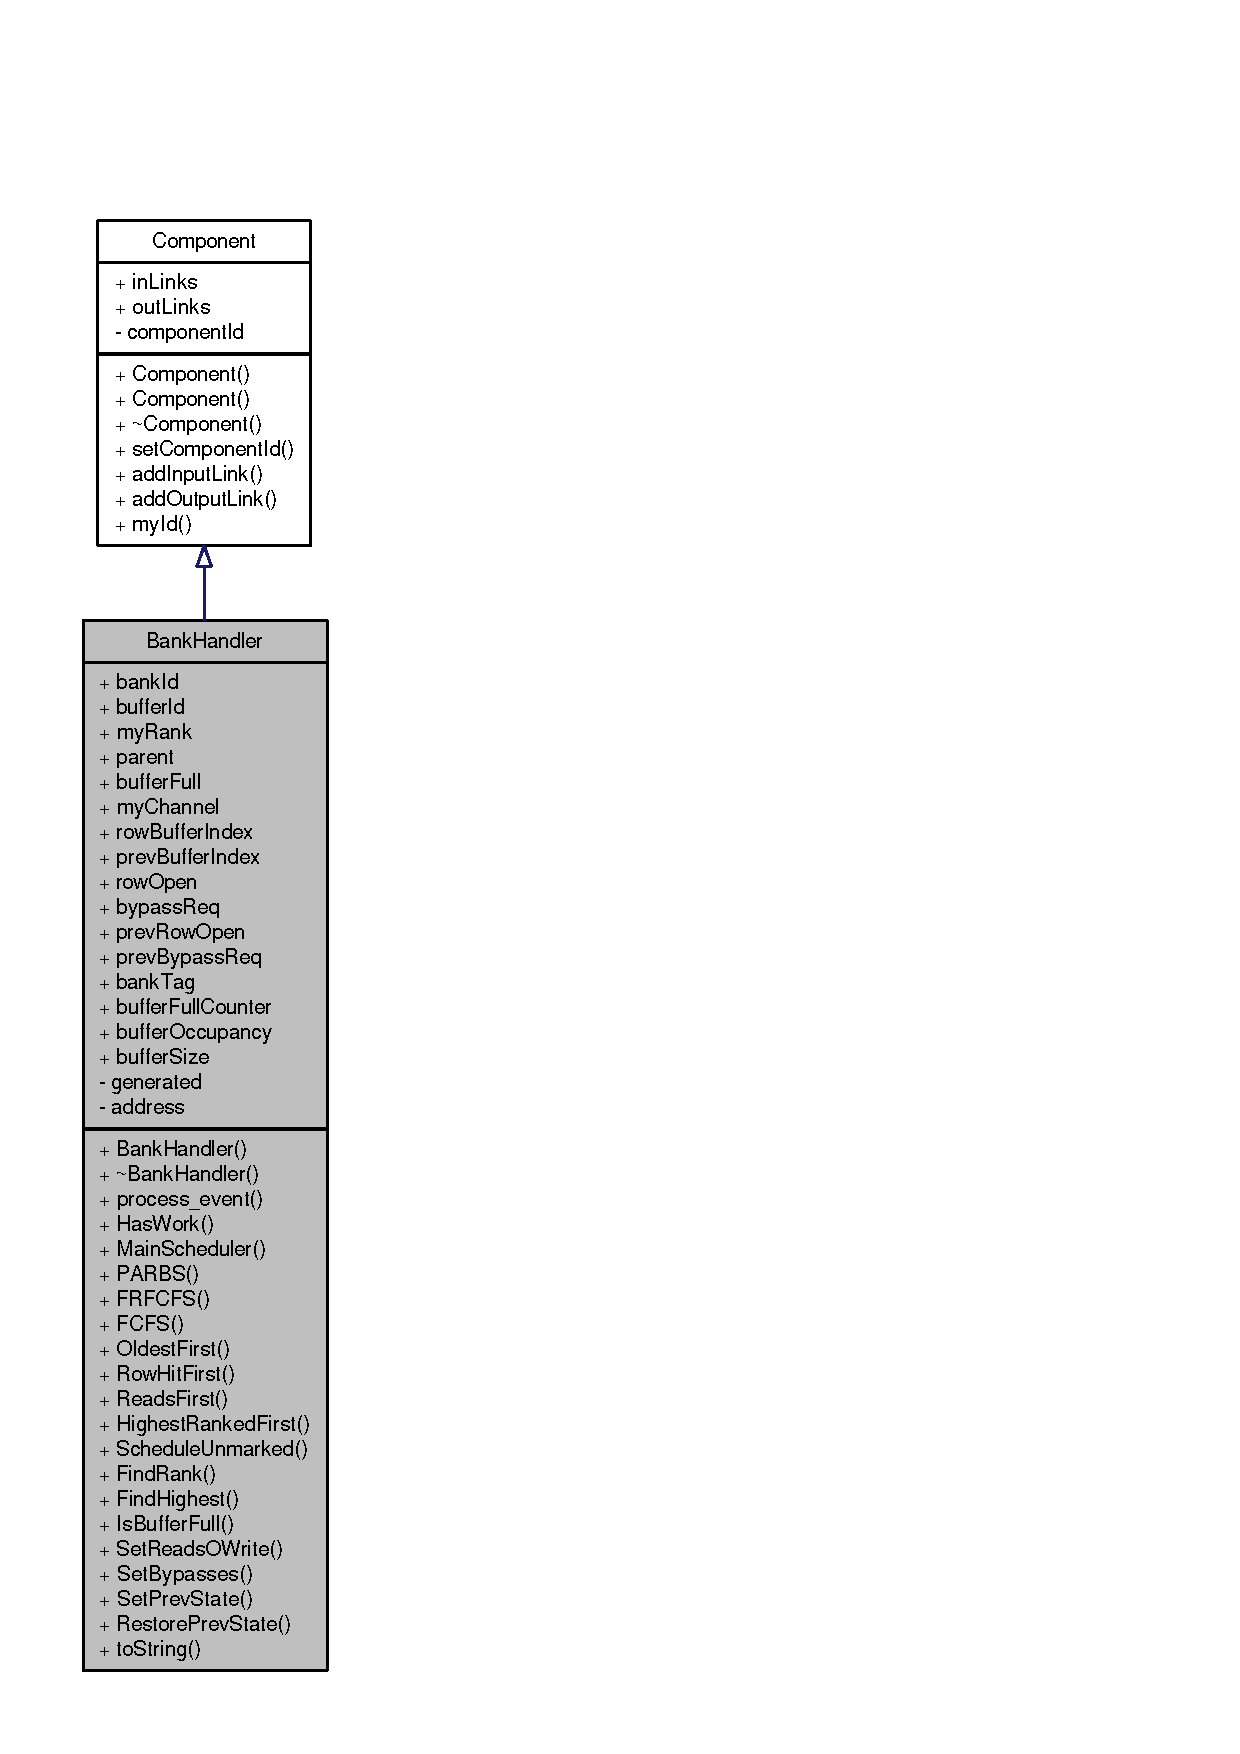
\includegraphics[height=400pt]{classBankHandler__inherit__graph}
\end{center}
\end{figure}
Collaboration diagram for BankHandler:\nopagebreak
\begin{figure}[H]
\begin{center}
\leavevmode
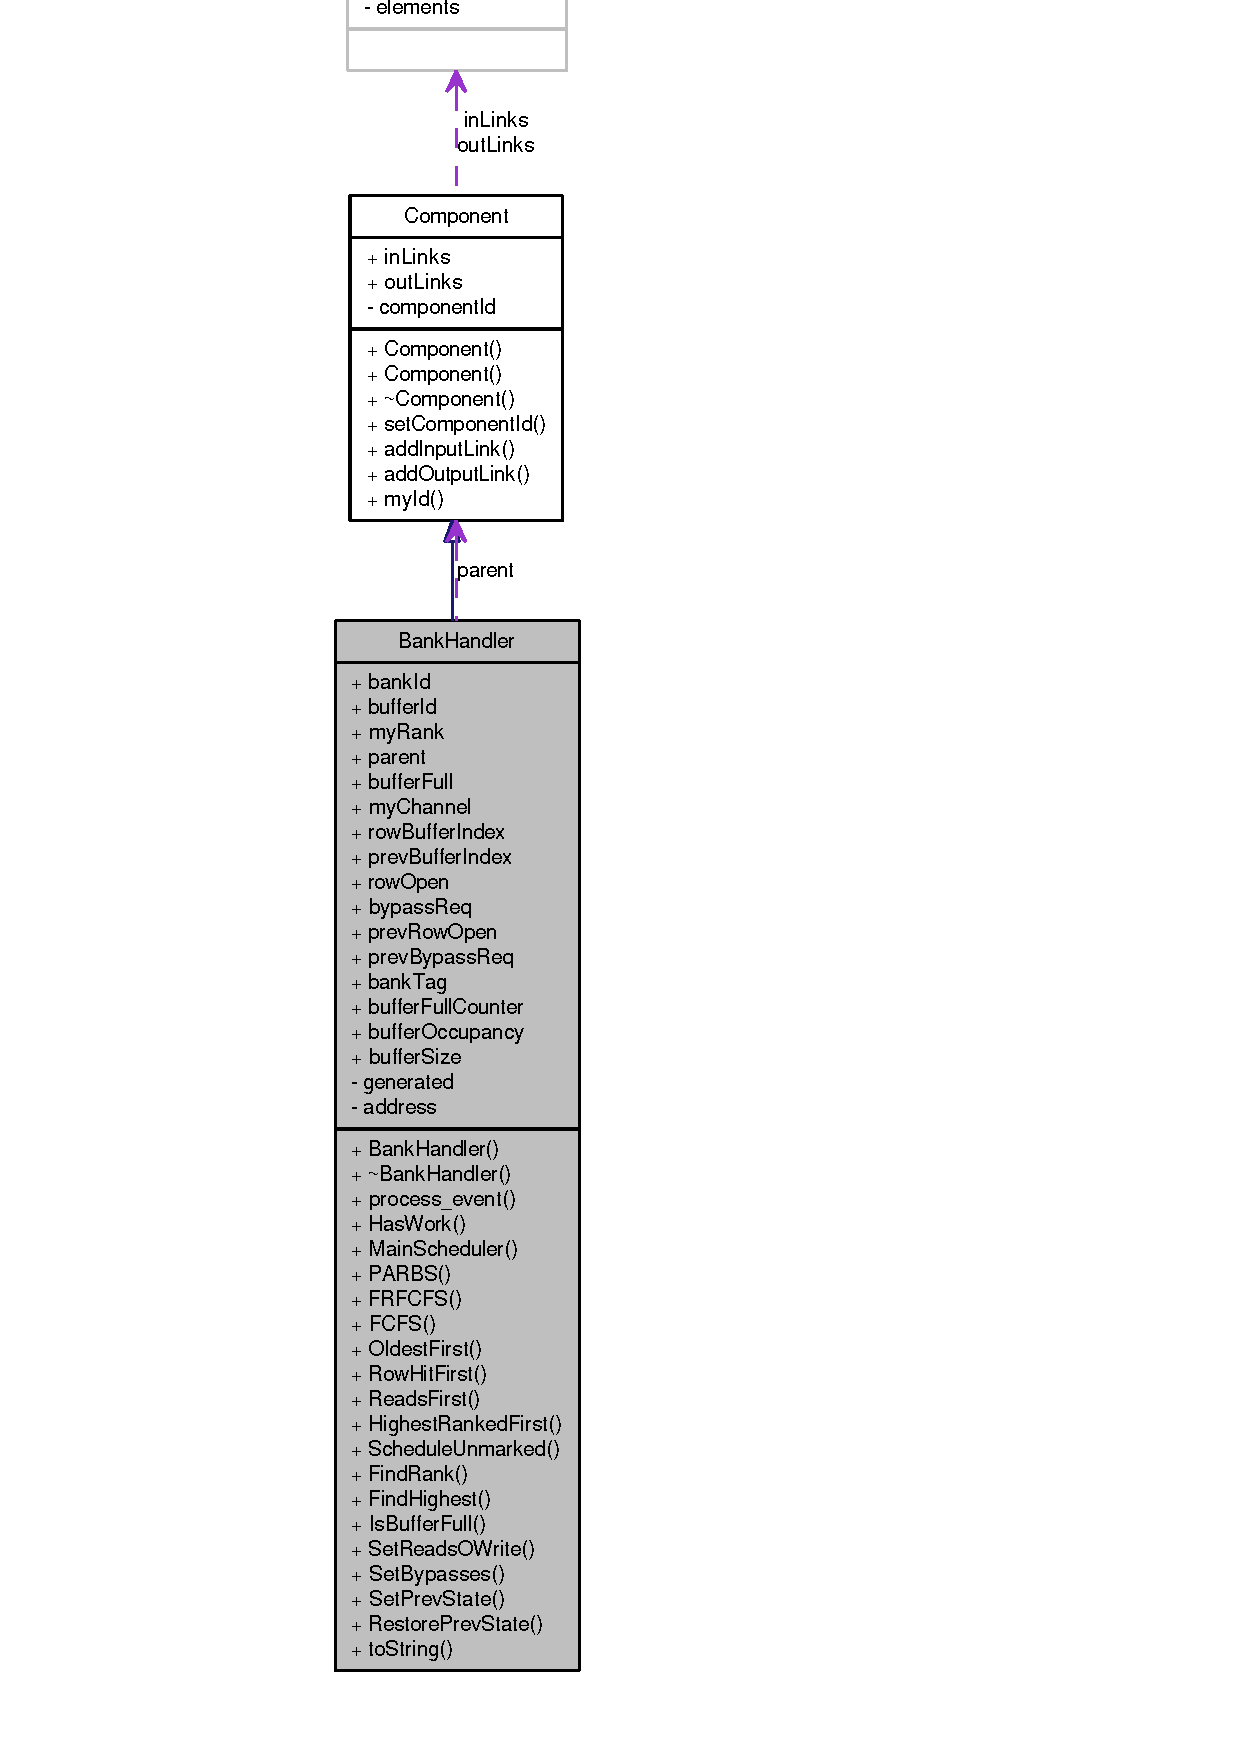
\includegraphics[height=400pt]{classBankHandler__coll__graph}
\end{center}
\end{figure}
\subsection*{Public Member Functions}
\begin{CompactItemize}
\item 
{\bf BankHandler} ()
\begin{CompactList}\small\item\em constructor \item\end{CompactList}\item 
{\bf $\sim$BankHandler} ()
\begin{CompactList}\small\item\em deconstructor \item\end{CompactList}\item 
void {\bf process\_\-event} ({\bf IrisEvent} $\ast$e)
\begin{CompactList}\small\item\em Main process function. \item\end{CompactList}\item 
bool {\bf HasWork} ()
\item 
bool {\bf MainScheduler} ({\bf Request} $\ast$req, int $\ast$index)
\begin{CompactList}\small\item\em The wrapper for all scheduling algorithms in this class. \item\end{CompactList}\item 
bool {\bf PARBS} ({\bf Request} $\ast$req, int $\ast$index)
\begin{CompactList}\small\item\em Function to implement PAR-BS scheduling policy. \item\end{CompactList}\item 
bool {\bf FRFCFS} ({\bf Request} $\ast$req, int $\ast$index)
\begin{CompactList}\small\item\em Function to implement FR-FCFS scheduling policy. \item\end{CompactList}\item 
bool {\bf FCFS} ({\bf Request} $\ast$req, int $\ast$index)
\begin{CompactList}\small\item\em Function to implement FCFS scheduling policy. \item\end{CompactList}\item 
bool {\bf OldestFirst} ({\bf Request} $\ast$req, int $\ast$index)
\begin{CompactList}\small\item\em Schedule oldest request. \item\end{CompactList}\item 
bool {\bf RowHitFirst} ({\bf Request} $\ast$req, int $\ast$index)
\begin{CompactList}\small\item\em Schedule row hits. \item\end{CompactList}\item 
bool {\bf ReadsFirst} ({\bf Request} $\ast$req, int $\ast$index)
\begin{CompactList}\small\item\em Schedule read request. \item\end{CompactList}\item 
bool {\bf HighestRankedFirst} ({\bf Request} $\ast$req, {\bf UInt} highest, int $\ast$index)
\begin{CompactList}\small\item\em Schedule highest ranked request. \item\end{CompactList}\item 
bool {\bf ScheduleUnmarked} ({\bf Request} $\ast$req, int $\ast$index)
\begin{CompactList}\small\item\em Schedule unmarked request. \item\end{CompactList}\item 
void {\bf FindRank} (int priority[$\,$])
\begin{CompactList}\small\item\em Set the rank of each request and return it in priority[]. \item\end{CompactList}\item 
{\bf UInt} {\bf FindHighest} ()
\begin{CompactList}\small\item\em Find the highest ranked request. \item\end{CompactList}\item 
bool {\bf IsBufferFull} ()
\begin{CompactList}\small\item\em Check whether the buffer is full or not. \item\end{CompactList}\item 
void {\bf SetReadsOWrite} ({\bf CallerType} caller, {\bf cache\_\-command} cmdType)
\begin{CompactList}\small\item\em Set the Reads over write counter in the current rank. \item\end{CompactList}\item 
void {\bf SetBypasses} (unsigned int index)
\begin{CompactList}\small\item\em Set the bypass counter in the current bank. \item\end{CompactList}\item 
void {\bf SetPrevState} ()
\begin{CompactList}\small\item\em Set the previous state. \item\end{CompactList}\item 
void {\bf RestorePrevState} ()
\begin{CompactList}\small\item\em Restore the previous state. \item\end{CompactList}\item 
std::string {\bf toString} ()
\end{CompactItemize}
\subsection*{Public Attributes}
\begin{CompactItemize}
\item 
{\bf UInt} {\bf bankId}
\begin{CompactList}\small\item\em Id of the bank in current rank. \item\end{CompactList}\item 
{\bf UInt} {\bf bufferId}
\begin{CompactList}\small\item\em Id of the buffer to look for. \item\end{CompactList}\item 
void $\ast$ {\bf myRank}
\begin{CompactList}\small\item\em pointer to its rank handler \item\end{CompactList}\item 
{\bf Component} $\ast$ {\bf parent}
\begin{CompactList}\small\item\em pointer to its request handler \item\end{CompactList}\item 
bool {\bf bufferFull}
\begin{CompactList}\small\item\em signal to indicate that the buffer is full \item\end{CompactList}\item 
{\bf UInt} {\bf myChannel}
\begin{CompactList}\small\item\em Id of the channel. \item\end{CompactList}\item 
{\bf UInt} {\bf rowBufferIndex}
\begin{CompactList}\small\item\em Index of current row in the row buffer. \item\end{CompactList}\item 
{\bf UInt} {\bf prevBufferIndex}
\begin{CompactList}\small\item\em Index of previous row in the row buffer (A temporary to restore previous state). \item\end{CompactList}\item 
bool {\bf rowOpen}
\begin{CompactList}\small\item\em Signal to indicate a row is open or not. \item\end{CompactList}\item 
unsigned int {\bf bypassReq}
\begin{CompactList}\small\item\em Counter of requests that have bypassed the first one. \item\end{CompactList}\item 
bool {\bf prevRowOpen}
\begin{CompactList}\small\item\em A temporary for row open to restore previous state. \item\end{CompactList}\item 
unsigned int {\bf prevBypassReq}
\begin{CompactList}\small\item\em Temporary of bypass counter. \item\end{CompactList}\item 
unsigned int {\bf bankTag}
\begin{CompactList}\small\item\em Counter to indicate the current tag. \item\end{CompactList}\item 
unsigned long long int {\bf bufferFullCounter}
\item 
unsigned long long int {\bf bufferOccupancy}
\item 
unsigned long long int {\bf bufferSize}
\end{CompactItemize}
\subsection*{Private Attributes}
\begin{CompactItemize}
\item 
bool {\bf generated}
\item 
{\bf uint} {\bf address}
\end{CompactItemize}


\subsection{Detailed Description}


Definition at line 49 of file bank\_\-handler.h.

\subsection{Constructor \& Destructor Documentation}
\index{BankHandler@{BankHandler}!BankHandler@{BankHandler}}
\index{BankHandler@{BankHandler}!BankHandler@{BankHandler}}
\subsubsection[{BankHandler}]{\setlength{\rightskip}{0pt plus 5cm}BankHandler::BankHandler ()}\label{classBankHandler_110a6818b5140e76f81476dc47bbfe1b}


constructor 



Definition at line 29 of file bank\_\-handler.cc.

References bufferFull, bufferFullCounter, bufferOccupancy, bufferSize, bypassReq, generated, prevBufferIndex, prevBypassReq, prevRowOpen, rowBufferIndex, and rowOpen.\index{BankHandler@{BankHandler}!$\sim$BankHandler@{$\sim$BankHandler}}
\index{$\sim$BankHandler@{$\sim$BankHandler}!BankHandler@{BankHandler}}
\subsubsection[{$\sim$BankHandler}]{\setlength{\rightskip}{0pt plus 5cm}BankHandler::$\sim$BankHandler ()}\label{classBankHandler_80d544db88459320e30adb73147123dd}


deconstructor 



Definition at line 52 of file bank\_\-handler.cc.

\subsection{Member Function Documentation}
\index{BankHandler@{BankHandler}!FCFS@{FCFS}}
\index{FCFS@{FCFS}!BankHandler@{BankHandler}}
\subsubsection[{FCFS}]{\setlength{\rightskip}{0pt plus 5cm}bool BankHandler::FCFS ({\bf Request} $\ast$ {\em req}, \/  int $\ast$ {\em index})}\label{classBankHandler_9fa196596e22b045d4dc68a20f9a9da3}


Function to implement FCFS scheduling policy. 



Definition at line 355 of file bank\_\-handler.cc.

References bufferId, myRank, OldestFirst(), and RankHandler::rbuffer.

Referenced by MainScheduler().

Here is the caller graph for this function:\nopagebreak
\begin{figure}[H]
\begin{center}
\leavevmode
\includegraphics[width=420pt]{classBankHandler_9fa196596e22b045d4dc68a20f9a9da3_icgraph}
\end{center}
\end{figure}
\index{BankHandler@{BankHandler}!FindHighest@{FindHighest}}
\index{FindHighest@{FindHighest}!BankHandler@{BankHandler}}
\subsubsection[{FindHighest}]{\setlength{\rightskip}{0pt plus 5cm}{\bf UInt} BankHandler::FindHighest ()}\label{classBankHandler_37259129fb6791f471c9113c4ddabaee}


Find the highest ranked request. 



Definition at line 550 of file bank\_\-handler.cc.

References MAX\_\-BUFFER\_\-SIZE, myRank, NO\_\-OF\_\-BUFFERS, NO\_\-OF\_\-THREADS, and RankHandler::rbuffer.

Referenced by PARBS().

Here is the caller graph for this function:\nopagebreak
\begin{figure}[H]
\begin{center}
\leavevmode
\includegraphics[width=420pt]{classBankHandler_37259129fb6791f471c9113c4ddabaee_icgraph}
\end{center}
\end{figure}
\index{BankHandler@{BankHandler}!FindRank@{FindRank}}
\index{FindRank@{FindRank}!BankHandler@{BankHandler}}
\subsubsection[{FindRank}]{\setlength{\rightskip}{0pt plus 5cm}void BankHandler::FindRank (int {\em priority}[$\,$])}\label{classBankHandler_4ce7b9b8cf98eb415bd944e3a3c2f388}


Set the rank of each request and return it in priority[]. 

\index{BankHandler@{BankHandler}!FRFCFS@{FRFCFS}}
\index{FRFCFS@{FRFCFS}!BankHandler@{BankHandler}}
\subsubsection[{FRFCFS}]{\setlength{\rightskip}{0pt plus 5cm}bool BankHandler::FRFCFS ({\bf Request} $\ast$ {\em req}, \/  int $\ast$ {\em index})}\label{classBankHandler_97cf9650294ab8a9e7cdd7f5c8fc1a53}


Function to implement FR-FCFS scheduling policy. 



Definition at line 337 of file bank\_\-handler.cc.

References bufferId, myRank, OldestFirst(), RankHandler::rbuffer, ReadsFirst(), and RowHitFirst().

Referenced by MainScheduler().

Here is the caller graph for this function:\nopagebreak
\begin{figure}[H]
\begin{center}
\leavevmode
\includegraphics[width=420pt]{classBankHandler_97cf9650294ab8a9e7cdd7f5c8fc1a53_icgraph}
\end{center}
\end{figure}
\index{BankHandler@{BankHandler}!HasWork@{HasWork}}
\index{HasWork@{HasWork}!BankHandler@{BankHandler}}
\subsubsection[{HasWork}]{\setlength{\rightskip}{0pt plus 5cm}bool BankHandler::HasWork ()}\label{classBankHandler_7990822a023b6ae8d6cf2f195900afd2}




Definition at line 237 of file bank\_\-handler.cc.

References bankId, and myRank.

Referenced by process\_\-event().

Here is the caller graph for this function:\nopagebreak
\begin{figure}[H]
\begin{center}
\leavevmode
\includegraphics[width=420pt]{classBankHandler_7990822a023b6ae8d6cf2f195900afd2_icgraph}
\end{center}
\end{figure}
\index{BankHandler@{BankHandler}!HighestRankedFirst@{HighestRankedFirst}}
\index{HighestRankedFirst@{HighestRankedFirst}!BankHandler@{BankHandler}}
\subsubsection[{HighestRankedFirst}]{\setlength{\rightskip}{0pt plus 5cm}bool BankHandler::HighestRankedFirst ({\bf Request} $\ast$ {\em req}, \/  {\bf UInt} {\em highest}, \/  int $\ast$ {\em index})}\label{classBankHandler_a4966de4e7e8d062be771c2382a55da6}


Schedule highest ranked request. 



Definition at line 515 of file bank\_\-handler.cc.

References bankId, Request::bankNo, bufferId, CLOSED, Request::cmdType, CONFLICT, HIGHEST\_\-RANKED\_\-FIRST, myRank, OPEN, RankHandler::rbuffer, rowBufferIndex, Request::rowNo, rowOpen, SetBypasses(), SetPrevState(), SetReadsOWrite(), Request::status, and Request::threadId.

Referenced by PARBS().

Here is the caller graph for this function:\nopagebreak
\begin{figure}[H]
\begin{center}
\leavevmode
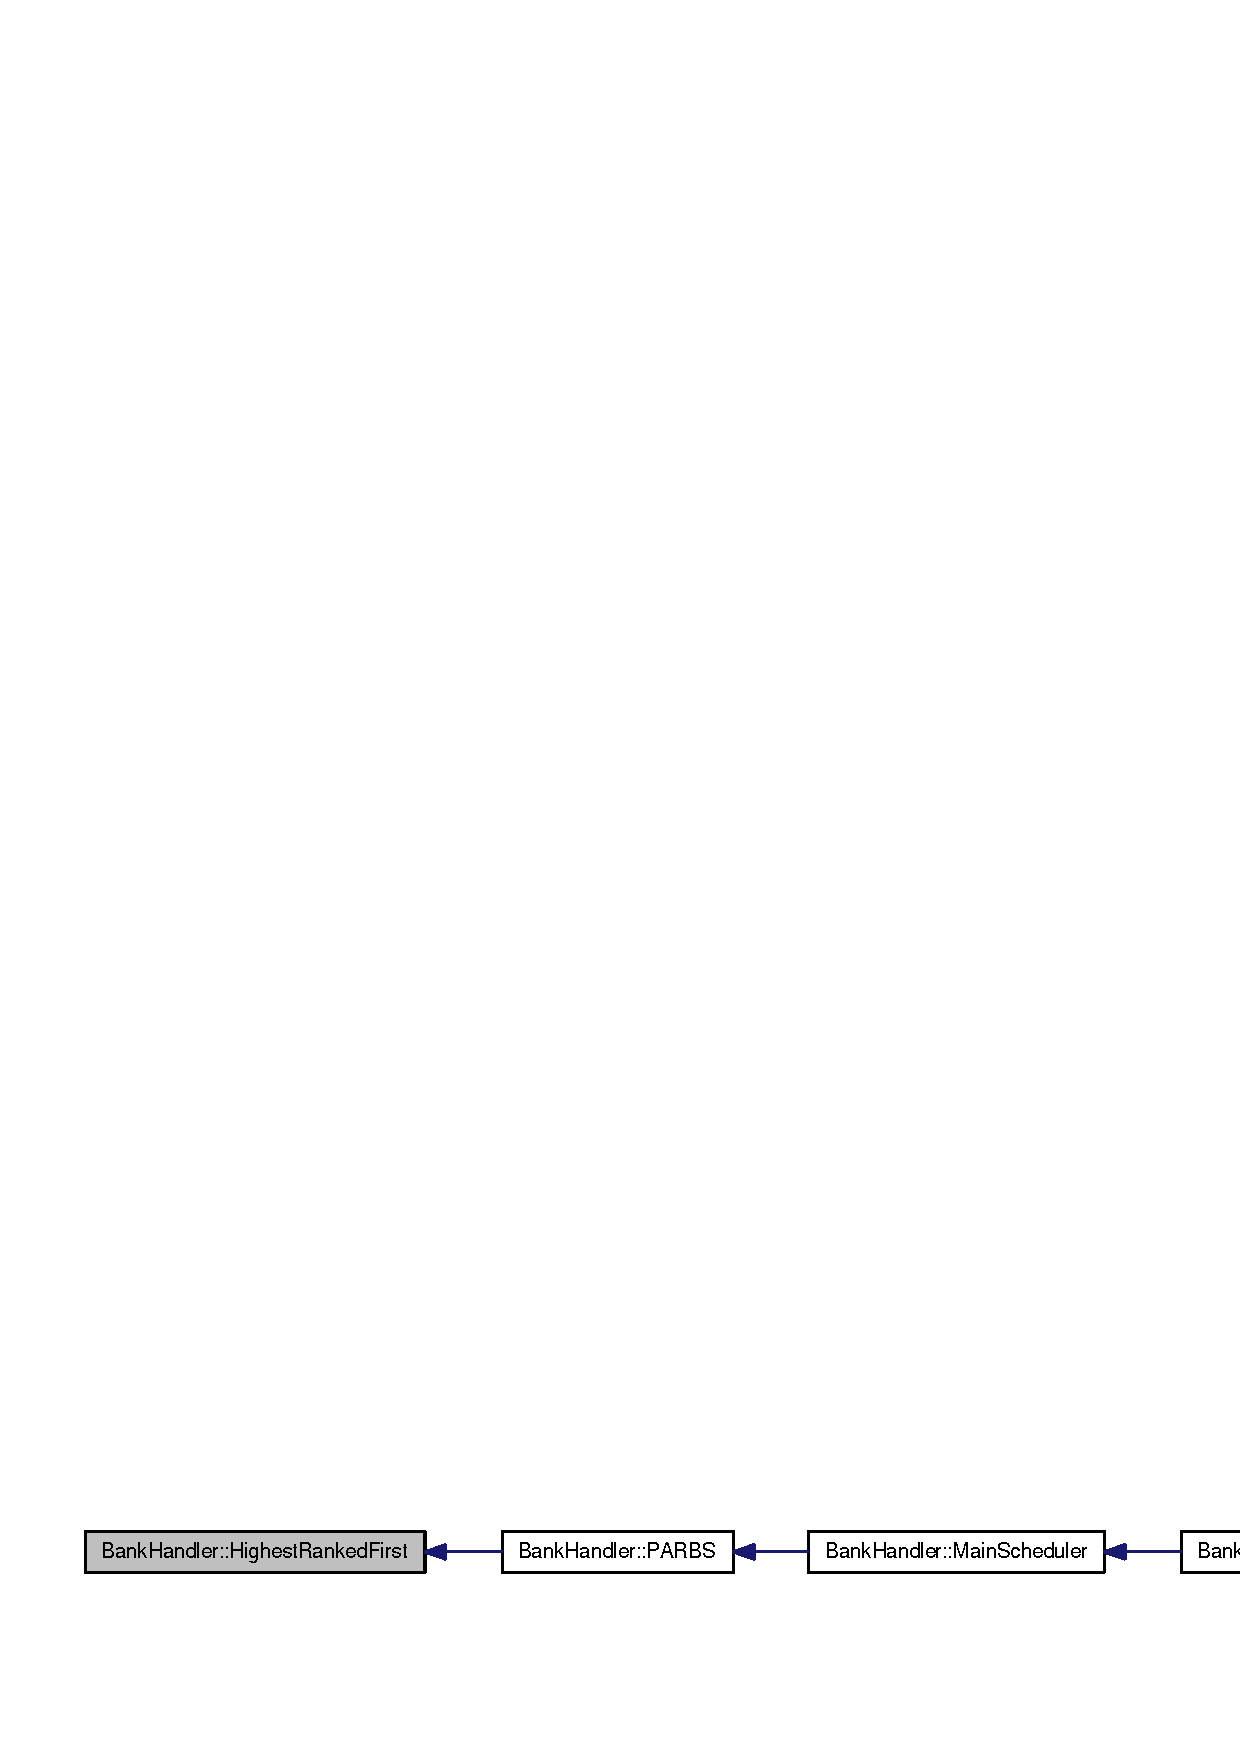
\includegraphics[width=420pt]{classBankHandler_a4966de4e7e8d062be771c2382a55da6_icgraph}
\end{center}
\end{figure}
\index{BankHandler@{BankHandler}!IsBufferFull@{IsBufferFull}}
\index{IsBufferFull@{IsBufferFull}!BankHandler@{BankHandler}}
\subsubsection[{IsBufferFull}]{\setlength{\rightskip}{0pt plus 5cm}bool BankHandler::IsBufferFull ()}\label{classBankHandler_5e6e874552e1b4e71589c489257b154b}


Check whether the buffer is full or not. 



Definition at line 245 of file bank\_\-handler.cc.

References bufferFull, bufferId, MAX\_\-BUFFER\_\-SIZE, and myRank.

Referenced by process\_\-event().

Here is the caller graph for this function:\nopagebreak
\begin{figure}[H]
\begin{center}
\leavevmode
\includegraphics[width=420pt]{classBankHandler_5e6e874552e1b4e71589c489257b154b_icgraph}
\end{center}
\end{figure}
\index{BankHandler@{BankHandler}!MainScheduler@{MainScheduler}}
\index{MainScheduler@{MainScheduler}!BankHandler@{BankHandler}}
\subsubsection[{MainScheduler}]{\setlength{\rightskip}{0pt plus 5cm}bool BankHandler::MainScheduler ({\bf Request} $\ast$ {\em req}, \/  int $\ast$ {\em index})}\label{classBankHandler_94d78e5801d1bba71f1ddb5405212d6c}


The wrapper for all scheduling algorithms in this class. 



Definition at line 261 of file bank\_\-handler.cc.

References CLOSE\_\-PAGE\_\-POLICY, dram\_\-page\_\-policy, FC\_\-FS, FCFS(), FR\_\-FCFS, FRFCFS(), mc\_\-scheduling\_\-algorithm, OPEN\_\-PAGE\_\-POLICY, PAR\_\-BS, and PARBS().

Referenced by process\_\-event().

Here is the caller graph for this function:\nopagebreak
\begin{figure}[H]
\begin{center}
\leavevmode
\includegraphics[width=420pt]{classBankHandler_94d78e5801d1bba71f1ddb5405212d6c_icgraph}
\end{center}
\end{figure}
\index{BankHandler@{BankHandler}!OldestFirst@{OldestFirst}}
\index{OldestFirst@{OldestFirst}!BankHandler@{BankHandler}}
\subsubsection[{OldestFirst}]{\setlength{\rightskip}{0pt plus 5cm}bool BankHandler::OldestFirst ({\bf Request} $\ast$ {\em req}, \/  int $\ast$ {\em index})}\label{classBankHandler_66cae2fc178c4ae45688198f4e02e8c8}


Schedule oldest request. 



Definition at line 372 of file bank\_\-handler.cc.

References bankId, Request::bankNo, bufferId, CLOSE\_\-PAGE\_\-POLICY, CLOSED, Request::cmdType, CONFLICT, dram\_\-page\_\-policy, myRank, OLDEST\_\-FIRST, OPEN, OPEN\_\-PAGE\_\-POLICY, RankHandler::rbuffer, rowBufferIndex, Request::rowNo, rowOpen, SetPrevState(), SetReadsOWrite(), and Request::status.

Referenced by FCFS(), FRFCFS(), and PARBS().

Here is the caller graph for this function:\nopagebreak
\begin{figure}[H]
\begin{center}
\leavevmode
\includegraphics[width=420pt]{classBankHandler_66cae2fc178c4ae45688198f4e02e8c8_icgraph}
\end{center}
\end{figure}
\index{BankHandler@{BankHandler}!PARBS@{PARBS}}
\index{PARBS@{PARBS}!BankHandler@{BankHandler}}
\subsubsection[{PARBS}]{\setlength{\rightskip}{0pt plus 5cm}bool BankHandler::PARBS ({\bf Request} $\ast$ {\em req}, \/  int $\ast$ {\em index})}\label{classBankHandler_b2357ebfa507e5e2837fb679d4ca498e}


Function to implement PAR-BS scheduling policy. 



Definition at line 312 of file bank\_\-handler.cc.

References bufferId, FindHighest(), HighestRankedFirst(), myRank, OldestFirst(), RankHandler::rbuffer, ReadsFirst(), RowHitFirst(), and ScheduleUnmarked().

Referenced by MainScheduler().

Here is the caller graph for this function:\nopagebreak
\begin{figure}[H]
\begin{center}
\leavevmode
\includegraphics[width=420pt]{classBankHandler_b2357ebfa507e5e2837fb679d4ca498e_icgraph}
\end{center}
\end{figure}
\index{BankHandler@{BankHandler}!process\_\-event@{process\_\-event}}
\index{process\_\-event@{process\_\-event}!BankHandler@{BankHandler}}
\subsubsection[{process\_\-event}]{\setlength{\rightskip}{0pt plus 5cm}void BankHandler::process\_\-event ({\bf IrisEvent} $\ast$ {\em e})}\label{classBankHandler_ff84a6f67d0bffbe69b069d7f2e718af}


Main process function. 



Definition at line 64 of file bank\_\-handler.cc.

References Request::address, bankId, Request::bankNo, bufferFull, bufferFullCounter, bufferOccupancy, bufferSize, CACHE\_\-PREFETCH, CACHE\_\-READ, CACHE\_\-WRITE, Request::cbufferInsertionTime, Request::channelNo, Request::cmdType, CONTINUE, IrisEvent::dst, IrisEvent::event\_\-data, generated, HasWork(), IsBufferFull(), MainScheduler(), myChannel, myRank, Simulator::Now(), parent, RequestHandler::process\_\-event(), ResponseHandler::process\_\-event(), CmdIssuer::process\_\-event(), PUSH\_\-BUFFER, RESPONSE\_\-BUFFER\_\-SIZE, Request::rowNo, Simulator::Schedule(), IrisEvent::src, START, Request::tag, and IrisEvent::type.

Referenced by AddrMap::process\_\-event().

Here is the caller graph for this function:\nopagebreak
\begin{figure}[H]
\begin{center}
\leavevmode
\includegraphics[width=420pt]{classBankHandler_ff84a6f67d0bffbe69b069d7f2e718af_icgraph}
\end{center}
\end{figure}
\index{BankHandler@{BankHandler}!ReadsFirst@{ReadsFirst}}
\index{ReadsFirst@{ReadsFirst}!BankHandler@{BankHandler}}
\subsubsection[{ReadsFirst}]{\setlength{\rightskip}{0pt plus 5cm}bool BankHandler::ReadsFirst ({\bf Request} $\ast$ {\em req}, \/  int $\ast$ {\em index})}\label{classBankHandler_e9a0e0abbb74e6f7b3d8de3421d3e81c}


Schedule read request. 



Definition at line 448 of file bank\_\-handler.cc.

References bankId, Request::bankNo, bufferId, CACHE\_\-PREFETCH, CACHE\_\-READ, CACHE\_\-WRITE, CLOSED, Request::cmdType, CONFLICT, MAX\_\-READ\_\-OV\_\-WRITE, myRank, OPEN, RankHandler::rbuffer, READS\_\-FIRST, RankHandler::readsOWrite, rowBufferIndex, Request::rowNo, rowOpen, SetBypasses(), SetPrevState(), SetReadsOWrite(), and Request::status.

Referenced by FRFCFS(), and PARBS().

Here is the caller graph for this function:\nopagebreak
\begin{figure}[H]
\begin{center}
\leavevmode
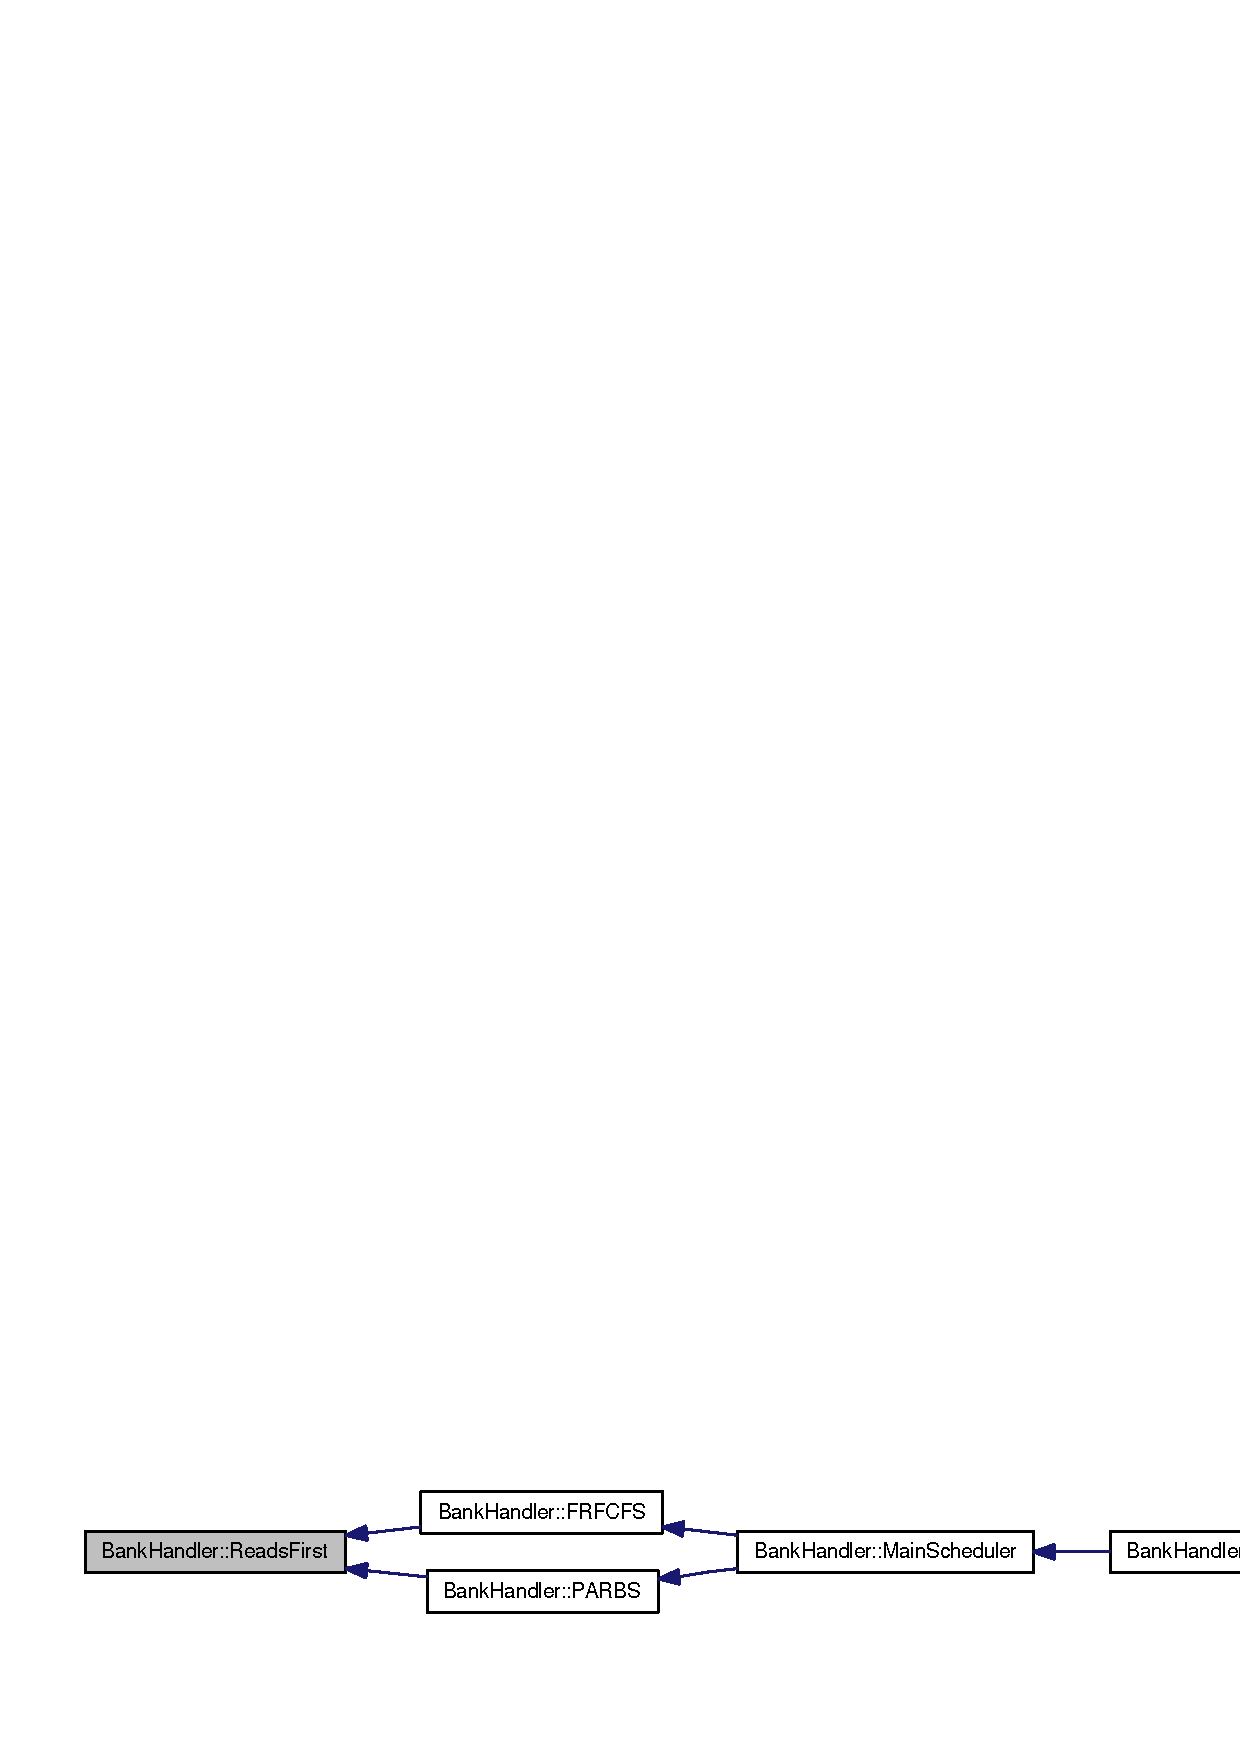
\includegraphics[width=420pt]{classBankHandler_e9a0e0abbb74e6f7b3d8de3421d3e81c_icgraph}
\end{center}
\end{figure}
\index{BankHandler@{BankHandler}!RestorePrevState@{RestorePrevState}}
\index{RestorePrevState@{RestorePrevState}!BankHandler@{BankHandler}}
\subsubsection[{RestorePrevState}]{\setlength{\rightskip}{0pt plus 5cm}void BankHandler::RestorePrevState ()}\label{classBankHandler_234ac01c0585c08d466b35b020607375}


Restore the previous state. 



Definition at line 658 of file bank\_\-handler.cc.

References bypassReq, myRank, prevBufferIndex, prevBypassReq, RankHandler::prevReadsOWrite, prevRowOpen, RankHandler::readsOWrite, rowBufferIndex, and rowOpen.\index{BankHandler@{BankHandler}!RowHitFirst@{RowHitFirst}}
\index{RowHitFirst@{RowHitFirst}!BankHandler@{BankHandler}}
\subsubsection[{RowHitFirst}]{\setlength{\rightskip}{0pt plus 5cm}bool BankHandler::RowHitFirst ({\bf Request} $\ast$ {\em req}, \/  int $\ast$ {\em index})}\label{classBankHandler_8efd50148051d7bab539f733defbc057}


Schedule row hits. 



Definition at line 413 of file bank\_\-handler.cc.

References bankId, Request::bankNo, bufferId, CLOSED, Request::cmdType, CONFLICT, HIT\_\-FIRST, myRank, OPEN, RankHandler::rbuffer, rowBufferIndex, Request::rowNo, rowOpen, SetBypasses(), SetPrevState(), SetReadsOWrite(), and Request::status.

Referenced by FRFCFS(), and PARBS().

Here is the caller graph for this function:\nopagebreak
\begin{figure}[H]
\begin{center}
\leavevmode
\includegraphics[width=420pt]{classBankHandler_8efd50148051d7bab539f733defbc057_icgraph}
\end{center}
\end{figure}
\index{BankHandler@{BankHandler}!ScheduleUnmarked@{ScheduleUnmarked}}
\index{ScheduleUnmarked@{ScheduleUnmarked}!BankHandler@{BankHandler}}
\subsubsection[{ScheduleUnmarked}]{\setlength{\rightskip}{0pt plus 5cm}bool BankHandler::ScheduleUnmarked ({\bf Request} $\ast$ {\em req}, \/  int $\ast$ {\em index})}\label{classBankHandler_4bc235f556be48bfd2d0f8432c43c8bd}


Schedule unmarked request. 



Definition at line 484 of file bank\_\-handler.cc.

References bankId, Request::bankNo, bufferId, CLOSED, Request::cmdType, CONFLICT, myRank, OPEN, RankHandler::rbuffer, rowBufferIndex, Request::rowNo, rowOpen, SetPrevState(), SetReadsOWrite(), Request::status, and UNMARKED\_\-FIRST.

Referenced by PARBS().

Here is the caller graph for this function:\nopagebreak
\begin{figure}[H]
\begin{center}
\leavevmode
\includegraphics[width=420pt]{classBankHandler_4bc235f556be48bfd2d0f8432c43c8bd_icgraph}
\end{center}
\end{figure}
\index{BankHandler@{BankHandler}!SetBypasses@{SetBypasses}}
\index{SetBypasses@{SetBypasses}!BankHandler@{BankHandler}}
\subsubsection[{SetBypasses}]{\setlength{\rightskip}{0pt plus 5cm}void BankHandler::SetBypasses (unsigned int {\em index})}\label{classBankHandler_d05b974c262629de52cf42219540f0e9}


Set the bypass counter in the current bank. 



Definition at line 630 of file bank\_\-handler.cc.

References bankId, bufferId, bypassReq, myRank, and RankHandler::rbuffer.

Referenced by HighestRankedFirst(), ReadsFirst(), and RowHitFirst().

Here is the caller graph for this function:\nopagebreak
\begin{figure}[H]
\begin{center}
\leavevmode
\includegraphics[width=420pt]{classBankHandler_d05b974c262629de52cf42219540f0e9_icgraph}
\end{center}
\end{figure}
\index{BankHandler@{BankHandler}!SetPrevState@{SetPrevState}}
\index{SetPrevState@{SetPrevState}!BankHandler@{BankHandler}}
\subsubsection[{SetPrevState}]{\setlength{\rightskip}{0pt plus 5cm}void BankHandler::SetPrevState ()}\label{classBankHandler_94781ff33ba7408091db65ec52d14fb9}


Set the previous state. 



Definition at line 649 of file bank\_\-handler.cc.

References bypassReq, myRank, prevBufferIndex, prevBypassReq, RankHandler::prevReadsOWrite, prevRowOpen, RankHandler::readsOWrite, rowBufferIndex, and rowOpen.

Referenced by HighestRankedFirst(), OldestFirst(), ReadsFirst(), RowHitFirst(), and ScheduleUnmarked().

Here is the caller graph for this function:\nopagebreak
\begin{figure}[H]
\begin{center}
\leavevmode
\includegraphics[width=420pt]{classBankHandler_94781ff33ba7408091db65ec52d14fb9_icgraph}
\end{center}
\end{figure}
\index{BankHandler@{BankHandler}!SetReadsOWrite@{SetReadsOWrite}}
\index{SetReadsOWrite@{SetReadsOWrite}!BankHandler@{BankHandler}}
\subsubsection[{SetReadsOWrite}]{\setlength{\rightskip}{0pt plus 5cm}void BankHandler::SetReadsOWrite ({\bf CallerType} {\em caller}, \/  {\bf cache\_\-command} {\em cmdType})}\label{classBankHandler_db51bdfe3e5dad885244280357c18f5f}


Set the Reads over write counter in the current rank. 



Definition at line 600 of file bank\_\-handler.cc.

References CACHE\_\-PREFETCH, CACHE\_\-READ, CACHE\_\-WRITE, HIGHEST\_\-RANKED\_\-FIRST, HIT\_\-FIRST, myRank, OLDEST\_\-FIRST, RankHandler::readsOWrite, and UNMARKED\_\-FIRST.

Referenced by HighestRankedFirst(), OldestFirst(), ReadsFirst(), RowHitFirst(), and ScheduleUnmarked().

Here is the caller graph for this function:\nopagebreak
\begin{figure}[H]
\begin{center}
\leavevmode
\includegraphics[width=420pt]{classBankHandler_db51bdfe3e5dad885244280357c18f5f_icgraph}
\end{center}
\end{figure}
\index{BankHandler@{BankHandler}!toString@{toString}}
\index{toString@{toString}!BankHandler@{BankHandler}}
\subsubsection[{toString}]{\setlength{\rightskip}{0pt plus 5cm}std::string BankHandler::toString ()}\label{classBankHandler_4d421b1df3349aeeeff7eb281de6c9b2}




Definition at line 256 of file bank\_\-handler.cc.

\subsection{Member Data Documentation}
\index{BankHandler@{BankHandler}!address@{address}}
\index{address@{address}!BankHandler@{BankHandler}}
\subsubsection[{address}]{\setlength{\rightskip}{0pt plus 5cm}{\bf uint} {\bf BankHandler::address}\hspace{0.3cm}{\tt  [private]}}\label{classBankHandler_bb566f9170d57d78537f4b518e1805f0}




Definition at line 103 of file bank\_\-handler.h.\index{BankHandler@{BankHandler}!bankId@{bankId}}
\index{bankId@{bankId}!BankHandler@{BankHandler}}
\subsubsection[{bankId}]{\setlength{\rightskip}{0pt plus 5cm}{\bf UInt} {\bf BankHandler::bankId}}\label{classBankHandler_9bf29827340b96477710c9a2636e7432}


Id of the bank in current rank. 



Definition at line 54 of file bank\_\-handler.h.

Referenced by HasWork(), HighestRankedFirst(), OldestFirst(), process\_\-event(), ReadsFirst(), RowHitFirst(), ScheduleUnmarked(), and SetBypasses().\index{BankHandler@{BankHandler}!bankTag@{bankTag}}
\index{bankTag@{bankTag}!BankHandler@{BankHandler}}
\subsubsection[{bankTag}]{\setlength{\rightskip}{0pt plus 5cm}unsigned int {\bf BankHandler::bankTag}}\label{classBankHandler_bbc313936f9271bc7f2a866c07188d2b}


Counter to indicate the current tag. 



Definition at line 90 of file bank\_\-handler.h.\index{BankHandler@{BankHandler}!bufferFull@{bufferFull}}
\index{bufferFull@{bufferFull}!BankHandler@{BankHandler}}
\subsubsection[{bufferFull}]{\setlength{\rightskip}{0pt plus 5cm}bool {\bf BankHandler::bufferFull}}\label{classBankHandler_61eaa92ca677fc7a5a4ae7eeca4e12e9}


signal to indicate that the buffer is full 



Definition at line 60 of file bank\_\-handler.h.

Referenced by BankHandler(), IsBufferFull(), and process\_\-event().\index{BankHandler@{BankHandler}!bufferFullCounter@{bufferFullCounter}}
\index{bufferFullCounter@{bufferFullCounter}!BankHandler@{BankHandler}}
\subsubsection[{bufferFullCounter}]{\setlength{\rightskip}{0pt plus 5cm}unsigned long long int {\bf BankHandler::bufferFullCounter}}\label{classBankHandler_0852159340fa8ed3cd24a3efd5e71523}




Definition at line 95 of file bank\_\-handler.h.

Referenced by BankHandler(), and process\_\-event().\index{BankHandler@{BankHandler}!bufferId@{bufferId}}
\index{bufferId@{bufferId}!BankHandler@{BankHandler}}
\subsubsection[{bufferId}]{\setlength{\rightskip}{0pt plus 5cm}{\bf UInt} {\bf BankHandler::bufferId}}\label{classBankHandler_59b546897a3e01e008c96baf74bf8c81}


Id of the buffer to look for. 



Definition at line 55 of file bank\_\-handler.h.

Referenced by FCFS(), FRFCFS(), HighestRankedFirst(), IsBufferFull(), OldestFirst(), PARBS(), ReadsFirst(), RowHitFirst(), ScheduleUnmarked(), and SetBypasses().\index{BankHandler@{BankHandler}!bufferOccupancy@{bufferOccupancy}}
\index{bufferOccupancy@{bufferOccupancy}!BankHandler@{BankHandler}}
\subsubsection[{bufferOccupancy}]{\setlength{\rightskip}{0pt plus 5cm}unsigned long long int {\bf BankHandler::bufferOccupancy}}\label{classBankHandler_bc0330e0fe0f24b18f17047ee794ea4b}




Definition at line 96 of file bank\_\-handler.h.

Referenced by BankHandler(), and process\_\-event().\index{BankHandler@{BankHandler}!bufferSize@{bufferSize}}
\index{bufferSize@{bufferSize}!BankHandler@{BankHandler}}
\subsubsection[{bufferSize}]{\setlength{\rightskip}{0pt plus 5cm}unsigned long long int {\bf BankHandler::bufferSize}}\label{classBankHandler_3ed4586984bfdc05e77334bccbe55d0d}




Definition at line 97 of file bank\_\-handler.h.

Referenced by BankHandler(), and process\_\-event().\index{BankHandler@{BankHandler}!bypassReq@{bypassReq}}
\index{bypassReq@{bypassReq}!BankHandler@{BankHandler}}
\subsubsection[{bypassReq}]{\setlength{\rightskip}{0pt plus 5cm}unsigned int {\bf BankHandler::bypassReq}}\label{classBankHandler_b30d5bf7f4e99ad9445a9bb046f26a0c}


Counter of requests that have bypassed the first one. 



Definition at line 87 of file bank\_\-handler.h.

Referenced by BankHandler(), RestorePrevState(), SetBypasses(), and SetPrevState().\index{BankHandler@{BankHandler}!generated@{generated}}
\index{generated@{generated}!BankHandler@{BankHandler}}
\subsubsection[{generated}]{\setlength{\rightskip}{0pt plus 5cm}bool {\bf BankHandler::generated}\hspace{0.3cm}{\tt  [private]}}\label{classBankHandler_9c9d3b2903e25e71b17c3273f05e0f48}




Definition at line 102 of file bank\_\-handler.h.

Referenced by BankHandler(), and process\_\-event().\index{BankHandler@{BankHandler}!myChannel@{myChannel}}
\index{myChannel@{myChannel}!BankHandler@{BankHandler}}
\subsubsection[{myChannel}]{\setlength{\rightskip}{0pt plus 5cm}{\bf UInt} {\bf BankHandler::myChannel}}\label{classBankHandler_71b1e66fc232b80db751d53caee7d7ad}


Id of the channel. 



Definition at line 83 of file bank\_\-handler.h.

Referenced by process\_\-event().\index{BankHandler@{BankHandler}!myRank@{myRank}}
\index{myRank@{myRank}!BankHandler@{BankHandler}}
\subsubsection[{myRank}]{\setlength{\rightskip}{0pt plus 5cm}void$\ast$ {\bf BankHandler::myRank}}\label{classBankHandler_d0ca9e41d498ef89fe2470aae4d87e6f}


pointer to its rank handler 



Definition at line 56 of file bank\_\-handler.h.

Referenced by FCFS(), FindHighest(), FRFCFS(), HasWork(), HighestRankedFirst(), IsBufferFull(), OldestFirst(), PARBS(), process\_\-event(), ReadsFirst(), RestorePrevState(), RowHitFirst(), ScheduleUnmarked(), SetBypasses(), SetPrevState(), and SetReadsOWrite().\index{BankHandler@{BankHandler}!parent@{parent}}
\index{parent@{parent}!BankHandler@{BankHandler}}
\subsubsection[{parent}]{\setlength{\rightskip}{0pt plus 5cm}{\bf Component}$\ast$ {\bf BankHandler::parent}}\label{classBankHandler_6c12437f421478ba8df1a0b45de47844}


pointer to its request handler 



Definition at line 57 of file bank\_\-handler.h.

Referenced by process\_\-event().\index{BankHandler@{BankHandler}!prevBufferIndex@{prevBufferIndex}}
\index{prevBufferIndex@{prevBufferIndex}!BankHandler@{BankHandler}}
\subsubsection[{prevBufferIndex}]{\setlength{\rightskip}{0pt plus 5cm}{\bf UInt} {\bf BankHandler::prevBufferIndex}}\label{classBankHandler_0ceaaf43fc1f868c17c3a7234b999d6b}


Index of previous row in the row buffer (A temporary to restore previous state). 



Definition at line 85 of file bank\_\-handler.h.

Referenced by BankHandler(), RestorePrevState(), and SetPrevState().\index{BankHandler@{BankHandler}!prevBypassReq@{prevBypassReq}}
\index{prevBypassReq@{prevBypassReq}!BankHandler@{BankHandler}}
\subsubsection[{prevBypassReq}]{\setlength{\rightskip}{0pt plus 5cm}unsigned int {\bf BankHandler::prevBypassReq}}\label{classBankHandler_1f79e0941b32431cdea572d7f43bd26a}


Temporary of bypass counter. 



Definition at line 89 of file bank\_\-handler.h.

Referenced by BankHandler(), RestorePrevState(), and SetPrevState().\index{BankHandler@{BankHandler}!prevRowOpen@{prevRowOpen}}
\index{prevRowOpen@{prevRowOpen}!BankHandler@{BankHandler}}
\subsubsection[{prevRowOpen}]{\setlength{\rightskip}{0pt plus 5cm}bool {\bf BankHandler::prevRowOpen}}\label{classBankHandler_569ae5a6b277a7176247337572904f7a}


A temporary for row open to restore previous state. 



Definition at line 88 of file bank\_\-handler.h.

Referenced by BankHandler(), RestorePrevState(), and SetPrevState().\index{BankHandler@{BankHandler}!rowBufferIndex@{rowBufferIndex}}
\index{rowBufferIndex@{rowBufferIndex}!BankHandler@{BankHandler}}
\subsubsection[{rowBufferIndex}]{\setlength{\rightskip}{0pt plus 5cm}{\bf UInt} {\bf BankHandler::rowBufferIndex}}\label{classBankHandler_dee67bbdd725a3645b6057ecfc8f68fd}


Index of current row in the row buffer. 



Definition at line 84 of file bank\_\-handler.h.

Referenced by BankHandler(), HighestRankedFirst(), OldestFirst(), ReadsFirst(), RestorePrevState(), RowHitFirst(), ScheduleUnmarked(), and SetPrevState().\index{BankHandler@{BankHandler}!rowOpen@{rowOpen}}
\index{rowOpen@{rowOpen}!BankHandler@{BankHandler}}
\subsubsection[{rowOpen}]{\setlength{\rightskip}{0pt plus 5cm}bool {\bf BankHandler::rowOpen}}\label{classBankHandler_69610e59acd2cf10bdeb3c6921f29094}


Signal to indicate a row is open or not. 



Definition at line 86 of file bank\_\-handler.h.

Referenced by BankHandler(), HighestRankedFirst(), OldestFirst(), ReadsFirst(), RestorePrevState(), RowHitFirst(), ScheduleUnmarked(), and SetPrevState().

The documentation for this class was generated from the following files:\begin{CompactItemize}
\item 
{\bf bank\_\-handler.h}\item 
{\bf bank\_\-handler.cc}\end{CompactItemize}
